\section{Particle Physics}
\subsection{Introduction}
I guess most of you are familiar with the elements of the periodic table. They can be distinguished from each other by the electric charge $Z_e$ on the atomic nucleus, and are also distinguishable by mass.

Some fundamental questions may then be asked. Are there other distinguishing properties of nuclei? Have the nuclei been in existence since the beginning of time? Why are some nuclei radioactive?

Nuclear physicists have long sought to answer these questions, and through their pursuit to unravel these once puzzling mysteries, particle physics was developed.

While it is often thought that the proton and neutrons are fundamental, elementary particles, this is not the case, and are rather structured entities. 

\subsubsection{Fermions and Bosons}
There are two classifications of the elementary particles of nature. They are:
\begin{enumerate}
\item Fermions
\item Bosons
\end{enumerate}

Fermions are particles which satisfy the \textbf{Pauli Exclusion Principle}: if an assembly of identical fermions is described in the terms of single-particle wave functions, then no two fermions can have the same wave-function. Electrons are such examples of fermions.The name "Fermions" was coined because fermions obeyed the Fermi-Dirac statistics of statistical mechanics.

Bosons, on the other hand, are so called, because they obey Bose-Einstein statistics. They are often characterised by the property that \emph{any} number of particles may be assigned the same single-particle wavefunction. As a result, in the case of bosons, coherent waves of macroscopic amplitude can be constructed, and may to a good approximation, be described with classical mechanics. An example of a boson, is a photon, and the corresponding classical field is the familiar electromagnetic field $\mathbf{E}$ and $\mathbf {B}$, which satisfy Maxwell's Equations.

At a more fundamental level, these properties are a consequence of the possible symmetries of the wave-function of a system of identical particles when the coordinates of any two particles are interchanged. In the case of fermions, \textbf{the wave-function changes sign}; it is antisymmetric. In the case of bosons, it is completely symmetric: the wave-function is unchanged.

There is also an observed relation between the angular momentum number (spin), \textit{s}, of a particle and its statistics. Do note that \textit{s} is quantised. For a fermion, \textit{s} takes on the values $\frac{1}{2},\frac{3}{2},\frac{5}{2}...$. For a boson, \textit{s} takes on the values $0,1,2,3...$

\subsubsection{The Picture of Nature}
Particle physics describes the world in terms of fermions, interacting through fields of which they are sources of. For example, the electron has a charge of $-e$ and produces an electromagnetic field $\mathbf{E}$ and $\mathbf{B}$, exerting force on other particles. The EM field, quantised according to the rules of quantum mechanics, correspond to the assembly of photons, which are bosons. Bose-Einstein statistics were first applied to photons.

There are four distinguishable types of interaction fields, as listed in table below.
\begin{table}[http]
\begin{center}
\begin{tabular}{|c|c|c|c|c|}
\hline Interaction Field & Boson & Spin & Strength & Theory \\ \hline
Gravitational Field & 'Gravitrons' Postulated & 2 & $10^{-42}$ & Chromodynamics \\
Weak Field & $W^+$, $W^-$, $Z$ particles & 1 & $10^{-2}$ & Flavordynamics\\
Electromagnetic Field & Photons & 1 & $10^{-13}$ & Electrodynamics\\
Strong Field & 'Gluons' Postulated & 1 & 10 & Geometrodynamics\\
\hline
\end{tabular}
\end{center}
\label{default}
\caption{The four interaction fields and their bosons and spins}
\end{table}

The electromagnetic force is one of the most important fundamental forces. For example, friction takes place when one object tries to slide over the surface of another. While the theory describing how frictional forces arise, it is fundamentally a consequence of the electromagnetic attraction between the atoms of one object and the other.

Without the electromagnetism there would be no friction and no tension, even no Van de Waals forces.

Particle physicists hope one day, they would be able to explain all forces with one fundamental force, and that idea will be described later.

While the force of gravitation and electromagnetism may be all so familiar, the weak and strong force would most likely appear new. This is because it was only recently discovered.

The range of the strong force is about $10^{-15}$m and that of the weak force is$10^{-17}$m. These ranges are even smaller than atomic sizes! For distances greater than this limit, the forces would become too small to be detectable. A proton on one side of the nucleus would be too far away from a proton on the other side to interact through the weak force!

All of the above interactions are fairly important in the study of nuclear physics and particle physics, although gravitation only becomes non-negligible in dense matter such as stars. Gravitational forces act on all particles and are important for the physics on the large scale of macroscopic bodies. On the small scale they are often negligible and will be ignored. This will be addressed later on.

There is an even greater diversity of elementary fermions than bosons.

It is convenient to divide the fermions into two classes: \emph{leptons} and \emph{quarks}. Leptons are not sources of strong fields and hence do not participate in the strong interaction. Quarks, on the other hand, participate in \textbf{all} interactions.

The electron is a good example of a lepton. Leptons and their interactions will be discussed later in chapter \ref{leptons::sec}

Quarks are always confined in compound systems which extend over distances of about 1fm. The term \emph{hadron} is generically used to refer to quark systems. The proton and neutron are hadrons, and so are mesons. Proton and neutron are the subject matter of chapter \ref{protonneutron::sec}

\subsubsection{Conservation laws and symmetries: Parity}
The total energy of an isolated system is constant in time. So are its linear and angular momentum. This should ring a bell, and are derivable from Newton's laws of motion, Maxwell's Equations and the laws of quantum mechanics.

This however, at a more fundamental level, can be seen to be the consequences of the symmetries of space and time. The law of conservation of linear momentum directly follows from the homogeneity of space, angular momentum from the isotropy of space; the direction of axes and origin for coordinate axes do not matter.

While these conservation laws are as significant in nuclear physics as elsewhere, there is another symmetry and conservation law that is of particular importance in quantum systems such as the nucleus: reflection symmetry and parity.

By reflection symmetry, we mean reflection about the origin:
\eqn{\v{r} \rightarrow \v{r}' = -\v{r}}

A single-particle wave-function is said to have a parity of $+1$ if it is even under reflection:
\eqn{\psi\brac{r}=\psi\brac{-r}}

It is said to have a parity of $-1$ if it is odd under reflection:
\eqn{\psi\brac{-r}=-\psi\brac{r}}

In the more general case, a many-particle wave-function has parity $+1$ if it is even under reflection of all the particle coordinates, and parity $-1$ if it is odd under reflection of all the particle coordinates.

It is important to understand the concept of parity well, because the laws of the electromagnetic and strong interaction are of exactly the same form if written in the left-handed and right-handed system. This is however, not true for the weak interaction. The weak interaction is often unimportant in the properties of atomic and nuclear systems. The wave-functions of these systems can be chosen to have to have a definite parity which does not change as the wave-function evolves in time according to the Schr\"{o}dinger Equation.

\subsubsection{Units}
In nuclear physics, the size of the nucleus makes $10^{-15} \text{ m } = 1 \text{ fm}$ (femtometre) convenient as a unit of length, usually referred to as a \emph{fermi}. Nuclear cross--sections, on the other hand, are measured in \emph{barns}; $1 \text{ b } = 10^{-28} \text{ m}^2 = 100 \text{ fm}^2$ as it has dimensions of area.

It is also convenient to measure energies in \emph{MeV}. It is also easier to quote masses by the units \emph{MeV/$c^2$}

For order--of--magnitude calculations, the masses of the electrons and protons, $m_e$ and $m_p$ respectively, may be taken as

\spliteqn{
m_e &\approx 0.5 MeV/c^2 \\
m_p &\approx 938 MeV/c^2
}

\subsection{The Standard Model}\label{StandardModel::sec}
This chapter provides a brief summary of the theories discussed in the rest of this book. This standard model describes all current understanding about the structure of matter. It gives us insight of how the universe was created. For the rest of this chapter, I shall discuss the ideas behind the standard model.

\subsubsection{The fundamental particles of matter}
Isn't it remarkable that the list of fundamental particles of matter can be listed in less that a tenth of this page? The number of fundamental particles have been reduced to a total of charge. 

The twelve particles are listed in table \ref{twelveparticles::table}. These twelve particles belong to the fermions, 6 quarks and 6 leptons.

\begin{table}[http]

\begin{center}
\begin{tabular}{|c c|c c |}
\hline
Quarks & Symbols & Leptons & Symbols \\ \hline
up & (u) & electron & ($e^-$) \\
down & (d) & electron--neutrino & ($v_e$) \\
strange & (s) & muon & ($\mu^-$) \\
charm & (c) & muon--neutrino & ($v_\mu$)\\
bottom  & (b) & tau & ($\tau^-$) \\
top & (u) & tau--neutrino & ($v_\tau$) \\ \hline

\end{tabular}
\end{center}
\caption{The Twelve Fundamental Particles}
\label{twelveparticles::table}
\end{table}

Already in this table, there is one familiar thing, and one surprise.

\subsubsection{Quarks}
Protons and neutrons, surprisingly, are not fundamental. They consists of \emph{quarks}.

Specifically, the proton is composed of two up quarks, and one down quark. The neutron on the other hand, is composed of two down quarks and one quark, We can write it it symbolically in this way:
\spliteqn{p \equiv uud\\
n \equiv udd}

Since the proton has a charge, this implies that quarks must be charged too. We can perform a simple solving for the simultaneous equation, derived from the charge of the proton and neutron, and their respective compositions:

\spliteqn{Q_u + Q_u +Q_d = 1\\
Q_u + Q_d + Q_d = 0\\
}

It follows that:

\fbox{The charge of an up quark is $Q_u = +\frac{2}{3}$ while the charge of a down quark is $Q_d = -\frac{1}{3}$}

If you recall your basic physics, charge was said to be quantised, in multiples of $1$, but in the standard model there are three basic quantities of charge: $+\frac{2}{3},-\frac{1}{3}\text{ ,and } -1$

Other quarks also have charges $+\frac{2}{3}$ and $-\frac{1}{3}$. These quarks are also shown in grouped into families and generations.

\begin{table}[http]
\begin{center}
\begin{tabular}{|c | c c c|}
\hline & 1st Generation & 2nd Generation & 3rd Generation \\ \hline
$+\frac{2}{3}$ & up & charm & top\\
$-\frac{1}{3}$ & down & strange & bottom \\ \hline
\end{tabular}
\end{center}
\label{quarkgroup::table}
\caption{Quarks Grouped by their Generation and Charge}
\end{table}%

While these quarks are grouped in roughly the order of discovery, it is grouped according how they interact to fundamental forces.

All the matter we see in the universe are protons and neutrons, and thus naturally there are more up and down quarks in the universe.

Note that the mass of quarks increase down the generation (i.e. the mass of the quarks in the first generation is smaller than that of the second generation). These heavier quarks were discovered by physicists when they collided particles are very high velocities, with enough energy to produce such a heavy quark.

During the formation of the universe, matter was very energetic so these heavier quarks had a greater role to play in the reactions that took place. As a result, physicists are trying to build large colliders to observe the behaviour of such quarks, allowing them to look back into the history of the universe.

\subsubsection{Leptons}
The familiar thing in the table previously is the electron, which is
one of the constituents of the atom and the particle that is
responsible for the electric current in wires. Electrons are
fundamental particles, which means that they are not composed of any
smaller particles -- they do not have any pieces inside them. All twelve
particles in table \ref{twelveparticles::table} are thought to be
fundamental --  they are all distinct and there are no pieces within them. 

It is fortunate that electrons is a familiar lepton. This is because the properties of the electron are mirrored in the muon and tau. There is very little, besides mass, that distinguishes the electron from the muon and tau. Their charge is the same, and the respond in a similar way to the fundamental forces. The only obvious difference between them is that the muon and tau are allowed to decay into other particles, while the electron is a stable particle.

Aside from making the number of leptons equal to the number of quarks, there seems to be no reason why the heavier leptons should exist. There are no apparent constraints on the existence of heavy leptons, while theories require heavy quarks exist (and they have already proven their existence). It is a matter of coincidence that there are equal number of quarks and leptons, and this is an area of question, which many physicists are exploring at this date.

The other three leptons are called neutrinos as they are electrically neutral. One must note that this is not equivalent to saying that the neutron is electrically neutral, because the neutron consists of quarks, which themselves have charge. Neutrinos on the other hand, are fundamental particles and are electrically neutral. From this stage on, we shall say that neutrinos are neutral, and that neutrons have zero charge.

The mass of neutrinos are amazingly small, even on the atomic scale. Experiments with the electron-neutrino suggest that it has a mass of less than one ten-thousanth of that of the electron. Many particle physicists believe that neutrinos are massless altogether.

The names chosen for the three neutrinos obviously demonstrate some link, between the charged leptons and themselves. This link is found in the way the leptons respond to one of the fundamental forces. This allows us to group the leptons in a similar way the quarks are grouped. 

\begin{table}[http]
\begin{center}
\begin{tabular}{|c|c c c|}
\hline & 1st Generation & 2nd Generation & 3rd Generation \\ \hline
$-1$ & electron & muon & tau \\ 
$0$ & electron--neutrino & muon--neutrino & tau--neutrino\\ \hline
\end{tabular}
\end{center}
\label{leptongroup::table}
\caption{Leptons Grouped by Generation and Charge}
\end{table}%

At this stage, we need to consider the forces by which all fundamental particles interact.

\subsubsection{The Four Fundamental Forces}
We already had a brief introduction to the four fundamental forces in the chapter of introduction. We shall now go through this more in depth, to understand why the quarks and leptons are grouped in such a fashion.

\subsubsection{The Strong Force}
Two protons placed a meter apart from each other would electrically repel $10^{42}$ times stronger than their gravitational attraction between them. This is due to their small mass. Over a similar distance the strong force would be effectively zero. But at the atomic scale, the strong force is at least equally great in magnitude as compared to the electromagnetic force. It is this strong force that packs the protons into a small volume, and resist being blown apart by the electromagnetic repulsive force.

As mentioned earlier in the chapter of introduction, the strong force acts only between quarks, and this distinguishes leptons from quarks. The leptons do not experience the strong force at all.

This strong force acting between quarks hold them together to form objects such as the proton and neutron. Leptons on the other hand do not feel this strong force, and as such do not bind together to form particles.
\begin{itemize}
  \item Quarks can \emph{only }bind together to form particles
  \item Leptons \textbf{DO NOT} bind together to form particles
\end{itemize}

Current theories of the strong force suggest that it is impossible to have a single quark isolated without any other quarks. All the quarks in the universe at the moment are bound up with others into particles. When we create new quarks in our experiments, they rapidly combine with others. This happens so quickly that it is impossible to ever see one on its own. The important experimental techniques are discussed later on on this book.

\subsubsection{The Weak Force}
The weak force is probably the most difficult of the fundamental forces to describe. This is because it least fits in our imagination what a force would do. The weak force does not attract or repel anything. It changes one particle into another. 

The weak force is the reason for the generation structure of the quarks and leptons. The weak force is felt by both quarks and leptons. In this respect it is the same as electromagnetic and gravitational forces -- the strong force is the only force felt by only one class of fermions. If two leptons come within range of the weak force, it is possible for them to change into other leptons. 

\begin{figure}[h]
\cen{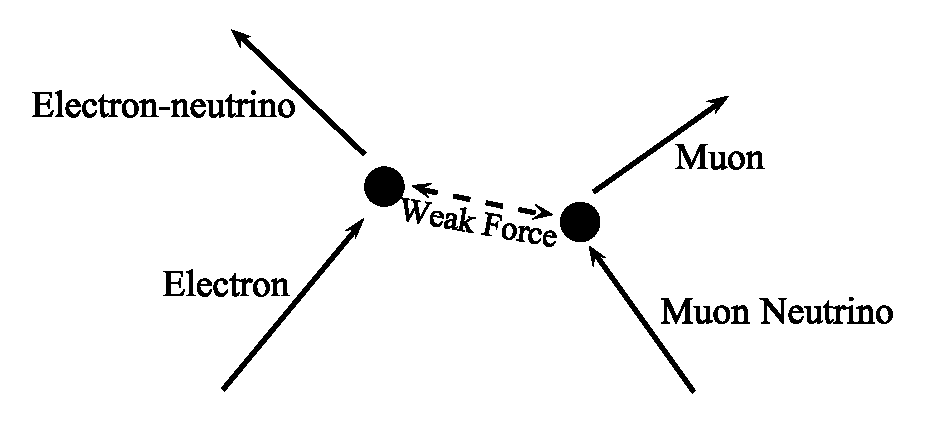
\includegraphics[scale=0.5]{images/WeakForce}
\label{weakforce::fig}
\caption{The effects of a weak force}}
\end{figure}

The electron can be turned into an electron-neutrino, and vice versa, but the electron cannot be turned into the muon-neutrino (or a muon for that matter). This is why we divide the leptons into generations. The weak force can act within the lepton generations, but not between them.

There is a slight complication when it comes to the quarks. Again the weak force can turn one quark into another and again the force acts within the generations of quarks. However, it is not true to say that the force cannot act across generations. It can, but with a much reduced effect.

As a result, one can say that the generations are not as strictly divided in the case of quarks as in the case of lepton and there is less of a generation gap between quarks.

\subsubsection{Bosons}
Just a quick recap. Bosons are particles:
\begin{enumerate}
\item that have a particle spin that is an integer number (1,2,3 etc.)
\item mediate the fundamental forces of physics under the quantum field theories
\end{enumerate}

\subsubsection{Photons}
Under the photon theory of light, a \emph{photon} is a discrete bundle of electromagnetic or light energy. Photons are usually always in motion, and travel at the speed of light.

In vacuum, the speed of photons is the 299792458 m $s^{-2}$.

Despite photons being a standard, fundamental particle, photons have zero mass and rest energy. Photons also carry energy and momentum, as described by the quantum theory formulae.
\eqn{E=hf \text{ and } p = \frac{h}{\lambda}} 
Where h is the planck's constant, $p$ is the momentum and $f$ is the frequency.

Contrary to popular belief, photons \textbf{can} be created and destroyed, and this occurs when radiation is absorbed and emitted.

The reason why photons were described as a fundamental particle rather than a wave, is because it can have particle-like interactions (i.e. collisions) with electrons and other particles, often known as the Compton effect. This is evident from Einstein's experiment, adopting the particle theory of light to explain the photoelectric effect.

Photons have a spin of $-1$ and are thus described as bosons. It has a spin axis parallel to that of its direction of travel (forward of backward pointing depending on the type of photon). This allows for the polarisation of light.

\subsubsection{Higgs Boson}
In the standard model, a hypothetical model called the \emph{Higgs Boson} was included. According to the standard model, space consists of a Higgs field, and in each point in space, there is a non-zero value. In this field, there are two neutral, and two charged components. One of the neutral components, and both charged components combine to form the W and Z bosons, in turn creating the weak force, described earlier.

The Higgs Boson has not been experimentally found yet, but the energy levels of which the Higgs Boson exist has been narrowed down, due to the experimental observations of the W bosons.

However, recently last year (2010), evidence at fermilab showed that there could be as many as 5 Higgs Bosons.

This concludes our chapter on the standard model.

\subsection{A Brief Introduction to Relativity}

\subsubsection{Momentum}
Momentum was initially proposed to be obtained from the formula $p=mv$. This is a familiar formula in Newtonian Mechanics, when dealing with classical mechanics.

However, tests were conducted to verify this formula. Note that under the force from a B-field on a charged particle is given by:
\eqn{F=q \brac{v\times B}}

Where $B$ is the strength of the magnetic field, $q$ is the charge of the particle and $v$ is the speed of the particle. The direction of the force vector, is obtained from the cross product, or by using Flemming's Left Hand Rule (which I find not very useful).

Anyway, let us proceed. Because the velocity vector and the force vector are orthogonal, the particle will move in a circular path. The magnitude of the velocity of the charged particle is also always constant.

\spliteqn{\frac{mv^2}{r} &= Bqv\\
\frac{mv}{r}&=Bq\\
r&=\frac{mv}{Bq}= \frac{p}{Bq}\\
p&=Bqr
}

A graph of $p$ was plotted against the velocity of the particle, in the case of the experiment, an electron. They were surprised to find that at speeds of light, the experimental results showed a somewhat exponential curve. Results fit Newtonian predictions closely at low speeds.

It was later found that the formula that correctly shows the data is:
\eqn{p=\frac{mv}{\sqrt{1-v^2/c^2}}}

Where in this case $p$ is the \textbf{relativistic momentum}. This is a radical discovery. It was difficult to see why Newton was wrong, because $p$, newtonian momentum, was defined to be obtained from the formula $mv$.

However, momentum is a very important and useful quantity, because it is a \textit{conservative} quantity. It allows us to simplify problems, and compare situations before and after time had past. In an isolated system, momentum is said to be conserved.

\subsubsection{Kinetic Energy}
Work done is calculated by this formula:
\eqn{W=F\cdot d}

Where $F$ is the force applied, and $d$ is the distance moved.

The work-energy theorem also tells us that
\eqn{\text{Work Done} = \text{ Change in Kinetic Energy}}

There are simple ways to calculate kinetic energy, $T$, with the mass of the particle and its velocity. The formula is given by:
\eqn{T=\frac{1}{2}mv^2 = \frac{p^2}{2m}}

Again, this was tested with a charged particle in an electric field, and Newtonian predictions were again wrong.

Einstein's theory showed the correct relationship to be:
\spliteqn{T&=\frac{mv^2}{\sqrt{1-v^2/c^2}}-mc^2\\
&=\brac{\gamma -1}mc^2
}

Where $\gamma$, is equal to 
\eqn{\gamma = \frac{1}{\sqrt{1-v^2/c^2}}}

Yet again, Newtonian predictions were close to the experimental results for kinetic energies at low velocities, and are therefore, "unviersally" true in the classical domain.

\subsubsection{Energy}
We have seen that energy can be calculated as follows:
\spliteqn{T=\brac{\gamma -1}mc^2 = \gamma mc^2 - mc^2}

Note that $\gamma$ is a function of velocity, while $mc^2$ is a fixed quantity. Therefore, If we were to accelerate a particle such that it's kinetic energy $T_1$ had been increased to $T_2$, then the energy supplied is given by the relationship:

\eqn{T_2-T_1=\gamma_1mc^2-\gamma_2mc^2}

The constant $mc^2$ had cancelled out!

\subsection{Quantum Mechanics}
In this section, we will go through the two most important experiments in physics.

\subsubsection{Double slit experiment}
This double slit experiment is key to the formation of quantum mechanics.

The idea is to direct a beam of electrons at a metal screen into which have been cut two rectangular slots. The slots are placed quite close to each other, closer than the width of the beam, and are very narrow. The electron beam can be produced in a very simple way using equipment similar to that found inside the tube of an ordinary television. However, an important addition is the ability to reduce the intensity of the beam so that the number of electrons per second striking the screen can be carefully controlled.

On the other side of the screen, and some distance away, is a device for detecting the arrival of electrons. This can be a sophisticated electronic device such as used in particle physics experiments, or it can be a simple photographic film (of very high sensitivity). The purpose of the experiment is to count the number of electrons arriving at different points after having passed through the slots in the screen.

The experiment is left running for some time and then the photographic film is developed. The exposed film shows a pattern of dark and light patches. In the negative, the dark patches are where electrons have arrived and exposed the film. The darker the patch is the greater the number of electrons that have arrived there during the experiment. A series of such exposures can be used to estimate the probability of an electron arriving at any given point.

This is a very significant experiment as the results disagree totally with oneÕs expectations if the classical theory is called upon to describe the results. 

In this case, however, fringes of alternating bright and dark appeared. This suggested the wave-particle duality of electrons. The bright fringes occur due to constructive interference, while the dark, because of destructive interference.

It is therefore often necessary to replace most of the laws of classical mechanics with that of quantum mechanics to explain the stability of atomic orbits and the discrete nature of atomic spectra.

At a sufficiently small scale, the wave--like nature of particles becomes non--negligible. In actual fact, we as humans have our own wavelengths too, but as we are relatively gigantic objects, our wave--like nature is not observable.

The fact that waves cannot be squeezed into an arbitrarily small volume without increasing indefinitely their frequency and thus their energy, preventing the collapse of electrons into the nucleus.

Another key experiment showing the wave nature of electrons, is the diffraction of electrons by a crystal. If an electron beam of momentum $\v{p}$passes through a crystal. These are the well known \emph{Bragg Reflections}.

A free particle of momentum $\v{p}$ is described by a field strength or \emph{wave--function}

\eqn{\psi_p\brac{\v{x},t} = e^{i\v{k}\v{x}-i\omega t}}

Where k is the \emph{wave vector} pointing into the direction of $\v{p}$ and $\omega$ is the \emph{wave frequency}.

\subsubsection{The Feynman Picture}
In the late 1940s, Richard Feynman decided that he could not relate
the traditional way of doing quantum mechanics, and tried to rethink
things for himself. He came up with a completely new way of doing
quantum mechanics. His technique involves a lot of mathematics,
although it is not exactly very mathematically rigorous, in the fact
that there was no such function produced previously to calculate
things. This is also known as the \emph{path integral formulation}. It
must be acknowledged, however, that it wasn't Feynman's original idea.
As far as I can recall, he was told of this at a bar by a friend.
Feynman went back, and formulated the entire theory in a single day.
Amazing, ain't he.

\subsection{Elementary Particle Dynamics}
In this chapter, \textbf{Feynman Diagrams} will be introduced, and the qualitative details of how particles interact will be discussed.

I refer you back to the table below:

\begin{table}[http]
\begin{center}
\begin{tabular}{|c|c|c|c|c|}
\hline Interaction Field & Boson & Theory \\ \hline
Gravitational Field & 'Gravitrons' Postulated & Chromodynamics \\
Weak Field & $W^+$, $W^-$, $Z$ particles & Flavordynamics\\
Electromagnetic Field & Photons & Electrodynamics\\
Strong Field & 'Gluons' Postulated & Geometrodynamics\\
\hline
\end{tabular}
\end{center}
\label{default}
\end{table}

I will be discussing the various theories qualitatively in this chapter.
\subsubsection{Quantum Electrodynamics}
Quantum Electrodynamics is by far, the most successful and simplest theory, which describes the electromagnetic processes. Most theories are built on Quantum Electrodynamics itself.

\emph{All electromagnetic phenomena can be reduced to the elementary process below:}

\cen{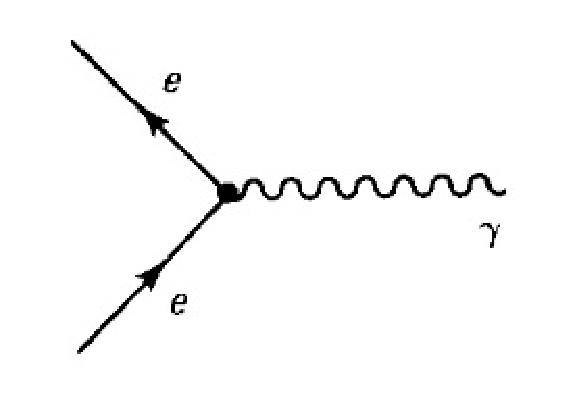
\includegraphics[scale=0.7]{images/QED}}


\subsection{Leptons and the Electromagnetic and Weak Interactions}\label{leptons::sec}

Leptons are objects that are easier to study (excluding the math). This is because it doesn't take part in the strong interactions that quarks do, and thus have more straightforward reactions as compared to quarks.

\subsubsection{Neutrinos}
The electron is a well-known particle, which properties should be already ingrained in your head (If it isn't I have nothing to say).

In any case, it has a counterpart called the \textbf{electron-neutrino}. This fundamental particle is common in nature. About $6\times10^{13}$ electron-neutrinos pass through a human every minute, but rest assured it is perfectly safe, since our body is transparent to these particles. Electron-neutrinos are produced through radioactive processes.

Muons, the second generation lepton, is produced in lab experiments. However, muons are massive and are thus unstable, decaying into electrons and neutrinos. They are not produced by radioactive decay, but rather observed in cosmic rays.

Tau-neutrinos and Taus are a rarity. There are not produced at this current time (\date) but was once produced frequently, when the universe was much more energetic (particle reactions would produce them). They are however, observed to exist through inference of certain particle reactions.

\begin{table}[http]
\begin{center}
\begin{tabular}{|c|c|c|}
\hline
1st Generation & 2nd Generation & 3rd Generation \\
\hline
Electron & Muon & Tau\\
$5.45\times10^{-4}M_p$ & $0.113 M_p$ & $1.90M_p$\\
\hline
Electron-neutrino & Muon-neutrino & Tau-neutrino\\
$2~3 \times 10^{-9} M_p$ & $<1.8\times 10^{-4}M_p$ & $1.9\times10^{-2}M_p$\\ \hline
\end{tabular}
\end{center}
\label{Neutrinos}
\caption{Properties of Lepton (Neutrinos)}
\end{table}%

The electron, muon and tau all have an electrical charge of -1 on our standard scale, while the three neutrinos do not have an electrical charge. Table 4.2 also shows that the charged leptons increase in mass from generation to generation. However, the neutrino masses are not so clear cut.

Our best experimental measurements have been unable to establish a definite mass for any of the neutrinos. It is not possible to capture just one example of a particle and place it on the scales. Masses have to be calculated by studying the ways in which the particles react. The more particles one measures, the more precise one can be about the size of their mass, causing the uncertainty.

For example, the tau-neutrino is a very rare object that is difficult to study. All we can say at this time is that its mass is less than 0.019 proton masses. This limit comes from studying the decay of the tau, which is itself a rare object. The uncertainty will become smaller as we measure more of them. The electron-neutrino, on the other hand, is much more common, so the upper limit on its mass is much more clearly defined.

Neutrinos seem like very weird particles. They may have no mass and they certainly have no charge, so they are very ghostly objects. Being leptons, they do not feel the strong force and having no electrical charge, they do not feel the electromagnetic force either. \textbf{The only way that neutrinos can interact is via the weak force.} (Ignoring gravity, which would be extremely weak for an individual neutrino. However, if there are enough neutrinos with mass in the universe, their combined gravity might stop the expansion of the universe.)

As weak force reactions are very rare, a particle that only reacts by the weak force cannot be expected to do very much. Estimates indicate that a block of lead 9 ? 1016 m thick would be required to significantly reduce the number of electron-neutrinos passing through your body at this moment.

\subsubsection{Neutrino Reactions with matter}
Neutrinos are difficult to use in experiments, but they are worth the effort for one reason: they are the only particles that allow a relatively uncluttered study of the weak force. After all, they do not react in any other way. Their reactions may be very rare, but if you have enough neutrinos to begin with then sufficient reactions can take place for a sensible study to be made.

Such an example of a reaction is as follows:
\eqn{v_e + n \rightarrow p+e^-}

This reaction has been of considerable experimental importance over the past few years. Astrophysicists have calculated the rate at which electron-neutrinos should be being produced by the sun. In order to check this theory physicists have, in several experiments, measured the number of neutrinos passing through the earth.

Note that if this neutron is part of an atom, it could transform one element into another. Eg.
\eqn{^{37}_{17}Cl + v_e \rightarrow ^{37}_{18}Ar + e^-}

The electron produced by the reaction would be moving too quickly to be captured by the argon nucleus. It would escape into the surrounding material. However, the transformation of a chlorine nucleus into an argon nucleus can be detected.

Theoretical calculations show that the number of reactions should be approximately 8 per second for every $10^{36}$ chlorine--37 atoms present in the tank. The experiment ran from 1968 to 1986 and over that time measured only 2 per second for every $10^{36}$ atoms in the tank. Both numbers represent incredibly small rates of reactions : a measure of how weak the weak force is. The conclusion is clear : the measured number of electron-neutrinos produced from the sun is totally different from the theoretical predictions. This is the solar neutrino problem.

\subsubsection{Aspects of the neutrino-neutron reaction}
The only way that a neutron can be turned into a proton is for one of the down quarks to be turned into an up quark. Evidently, inside the neutron, the following reaction has taken place:
\eqn{v_e+d\rightarrow u + e^-}

The other two quarks are unaffected. This is due to the short range of the weak force. The neutrino has to enter the neutron and pass close to one of the quarks within it for the reaction to be triggered.
The up and down quarks are different particles with different electrical charges. Examining the reaction more carefully by observing the individual charges of the particles, we see that \textbf{charge is conserved}.
%\subsubsection{Electromagnetic Interaction} 
%The electromagnetic field is most conveniently described by a vector potential $\v{A}$ and a scalar potential $\phi$. For simplicity, we consider only the potential $\phi\brac{\v{r}, t}$. Applying the Maxwell's Equations, this may be chosen to satisfy the wave-equation:
%\eqn{\nabla^2\phi - \frac{1}{c^2}\pdd{\phi}{t} =-\frac{\rho\brac{\v{r},t}}{\epsilon_0}}